% --------------------------------------------------------------------------------------------------
% Section: Results
% --------------------------------------------------------------------------------------------------

% Main section for presenting experiment outcomes
\section{Results} 

% --------------------------------------------------------------------------------------------------
% Subsection: Training Time and Performance
% --------------------------------------------------------------------------------------------------

\subsection{Training Time and Performance} 

% Description of training setup: model, hardware, and environment
The lung cancer detection model, based on the ResNet50 architecture, was trained on a labeled 
dataset of medical lung images. The training process was conducted using a traditional CPU-based 
environment. The system used for training included an Intel Core i7 processor with 10 cores, and 
training was completed over 20 epochs.

% Table to present training metrics, [H] forces it to appear 'Here' (float package required)
\begin{table}[H] 
\centering
\begin{tabular}{|c|c|} % Two-column table with vertical borders
\hline
\textbf{Metric} & \textbf{Value} \\ % Header row
\hline
Processor & Intel Core i7 \\ % Hardware specs
Cores/Threads & 10 Cores / 16 Threads \\
Training Time (Total) & 5 hours 20 minutes \\ % Total time for 20 epochs
Average Time per Epoch & 12.8 minutes \\ % Mean epoch time
\hline
\end{tabular}
\caption{Training Summary of CPU} % Table caption
\end{table}

% Explanation about CPU performance limitations for training deep models
While the CPU successfully completed the training task, it required several hours due to the 
computational intensity of deep convolutional neural networks like ResNet50. This highlights the 
limitations of using CPUs for large-scale deep learning tasks, particularly in terms of training 
time.

% Figure comparing training times
\vspace{1em}
\begin{center} 
    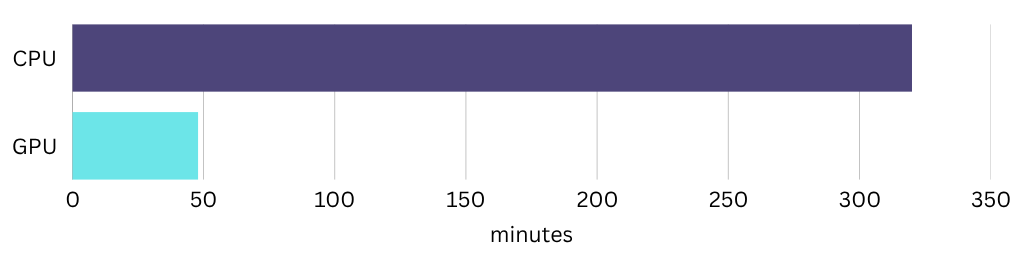
\includegraphics[width=\textwidth]{../assets/07-results/graph-cpu-vs-gpu.png} 
    \small\textit{Chart comparison of training time between GPU and CPU.} 
\end{center}
\vspace{1em} 

% --------------------------------------------------------------------------------------------------
% Subsection: Theoretical GPU Performance (Compared to CPU)
% --------------------------------------------------------------------------------------------------

\subsection{Theoretical GPU Performance (Compared to CPU)}

% Discussion of GPU strengths for deep learning tasks
Although the training was conducted on a CPU, it is important to consider the theoretical 
performance advantages of GPUs. Graphics Processing Units (GPUs) are highly optimized for parallel 
floating-point computations, which are common in deep learning tasks. The performance of GPUs is 
often measured in TFLOPS (Tera Floating Point Operations Per Second).

% --------------------------------------------------------------------------------------------------
% Subsubsection: Effective TFLOPS Calculation
% --------------------------------------------------------------------------------------------------

% Unnumbered subsubsection for showing the formula
\subsubsection*{Effective TFLOPS Calculation} 

% Formula for calculating FLOPS
\[
\text{FLOPS} = \text{Number of Cores} \times \text{Clock Speed (Hz)} \times \text{FLOPs per Cycle}
\]

% Conversion from FLOPS to TFLOPS
\[
\text{TFLOPS} = \frac{\text{FLOPS}}{10^{12}}
\]

% Example calculation using GPU specs
For example, a GPU with:
\begin{itemize}
    \item 8704 CUDA cores
    \item Clock speed of 1.7 GHz
    \item 2 FLOPs per core per cycle
\end{itemize}

would yield:

% FLOPS calculation with example values
\[
\text{FLOPS} = 8704 \times 1.7 \times 10^9 \times 2 = 29.6 \times 10^{12} = 29.6 \text{ TFLOPS}
\]

% Note on how this compares to CPU performance
This is several orders of magnitude higher than a standard CPU, which may reach only up to 0.5–1.5 
TFLOPS under optimal conditions.

% TFLOPS comparison image
\vspace{1em} 
\begin{center} 
    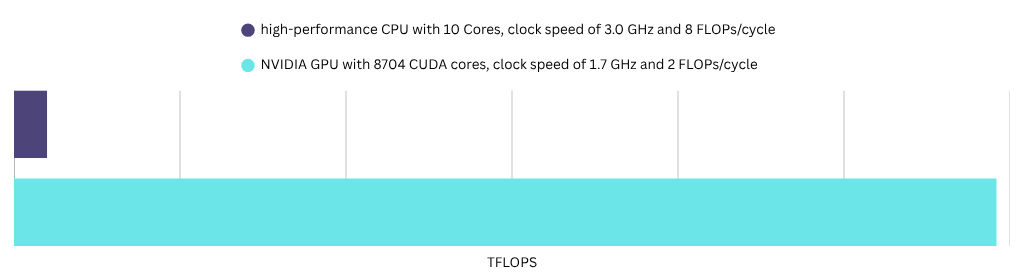
\includegraphics[width=\textwidth]{../assets/07-results/tflops-cpu-vs-gpu.png} 
    \small\textit{Chart comparison of TFLOPS values between GPU and CPU.} 
\end{center}
\vspace{1em} 

% --------------------------------------------------------------------------------------------------
% Subsection: Components Influencing Training Speed
% --------------------------------------------------------------------------------------------------

\subsection{Components Influencing Training Speed}

% List of hardware/software factors that affect model training speed
Several hardware and software factors significantly influence deep learning training performance:

\begin{itemize}
    \item \textbf{Core Count and Parallelism} – More cores allow parallel execution of matrix 
    operations. % Critical for speeding up tensor operations

    \item \textbf{Clock Speed} – Higher frequencies can increase operation speed, but also power 
    consumption. % Affects throughput but with trade-offs

    \item \textbf{Memory Bandwidth} – High-speed memory access is critical for transferring large 
    tensors during training. % Prevents memory bottlenecks

    \item \textbf{Cache Size and Architecture} – Affects the ability to reuse data without frequent 
    memory access. % Important for temporal locality of data

    \item \textbf{Software Optimization} – Efficient usage of libraries such as PyTorch with 
    multithreading and vectorization can impact performance greatly. 
    % Code-level tuning makes majorimpact
\end{itemize}
